\documentclass[letterpaper,12pt,fleqn]{article}
\usepackage{matharticle}
\usepackage{siunitx}
\pagestyle{plain}

\begin{document}

\begin{center}
  \large
  Math-13 Sections 01, 02

  \Large
  Final Exam \#2

  Due: 12/3/2020 at 10:00pm
\end{center}

\vspace{0.5in}

This exam is open book and notes.  You may use a calculator.  No collaboration or other web access is allowed. All
answers must be in exact form unless stated otherwise (i.e., no decimal answers allowed).  You \emph{must} show all
work and that work must be logical and complete; there is \emph{no} credit for guessed answers or answers without
supporting work.

You must work the exam problems, in order, on separate sheets of paper; camscan your results into a single PDF
file; and then submit your PDF file back to Moodle (just like the written homeworks and midterm exams).  This
\emph{must} be done by the deadline; late exams, multiple file or non-PDF submissions, and exams sent by email will
not be accepted.

Good luck!

\vspace{0.5in}

\begin{enumerate}[left=0pt,itemsep=0.5in]

\item Evaluate the following:
  \begin{enumerate}
  \item \(\displaystyle\int (3x^2-5x+2)dx\)
  \item \(\displaystyle\int_1^2 (3x^2-5x+2)dx\)
  \end{enumerate}

\item A certain vaccine is created by mixing a certain retrovirus with a certain protein in a large vat.  When the
  reactants are first mixed together, the amount of vaccine produced is accelerating at a rate of
  \SI{2}{grams/hour^2}.  Assuming that the initial rate of production is \SI{0}{grams/hour} and the vat is
  initially seeded with \SI{10}{grams} of pre-made vaccine, how much vaccine does the vat contain after
  \SI{24}{hours}?

  \newpage

\item Consider the following function (assume that the curved parts are semicircles):
  \begin{center}
    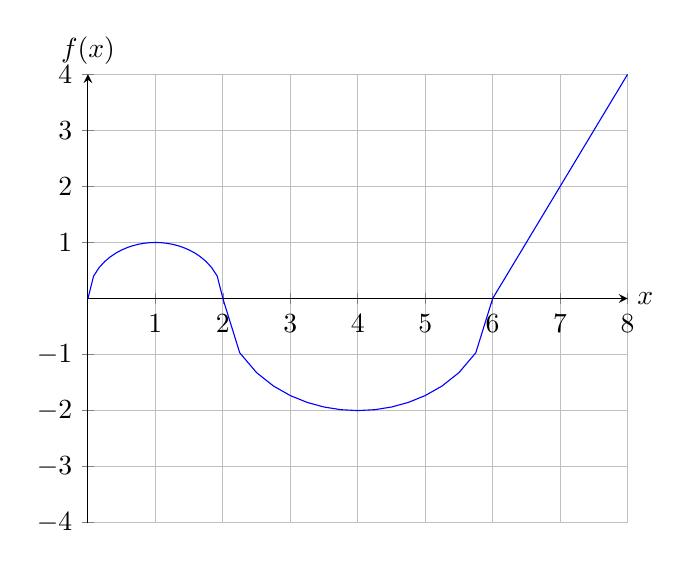
\begin{tikzpicture}
      \begin{axis}[
          axis lines=middle,
          grid=both,
          xmin=0,
          xmax=8,
          ymin=-4,
          ymax=4,
          xtick distance=1,
          ytick distance=1,
          xlabel={\(x\)},
          ylabel={\(f(x)\)},
          x label style={at={(axis cs:8,0)},anchor=west},
          y label style={at={(axis cs:0,4)},anchor=south},
          clip=false
        ]
        \addplot [domain=0:2,blue] {sqrt(1-(x-1)^2)};
        \addplot [domain=0:6,blue] {-sqrt(4-(x-4)^2)};
        \addplot [domain=6:8,blue] {2*x-12};
      \end{axis}
    \end{tikzpicture}
  \end{center}
  Calculate \(\displaystyle\int_0^8f(x)dx\).  Your answer must be in exact form (no decimals).

\item Let \(\int_0^2f(x)dx=3\) and \(\int_0^2g(x)dx=-2\).  Calculate:
  \[\int_0^2[5f(x)-2g(x)+1]dx\]

\item Estimate \(\int_1^7x^3dx\):
  \begin{enumerate}
  \item Using a left-hand Riemann sum with \(n=6\).
  \item Using a right-hand Riemann sum with \(n=6\).
  \end{enumerate}

\item Calculate the exact value for \(\int_1^7x^3dx\).

  \newpage

\item Calculate the following sums.  Your score will be based on how efficiently you perform the calculations.  Note
  that there is NO credit for manually adding all of the terms (which would take a long time anyway).
  \begin{enumerate}
  \item \(\displaystyle\sum_{k=1}^{100}(2k+1)\)
  \item \(\displaystyle\sum_{k=1}^{100}[k^3-(k+1)^3]\)
  \end{enumerate}

\item Let \(\displaystyle f(x)=\int_{x^2}^\pi(x^2\sqrt{x+1}+5)dx\).  Determine \(f'(x)\).

\item Let \(f(x)=3x(x^2+1)^3\).  What is the average value of \(f(x)\) on \([0,2]\)?

\item Evaluate: \(\displaystyle\int_4^{12}x\sqrt{2x+1}dx\).

\end{enumerate}

\end{document}
